\documentclass[english,svgnames,notes=hide,14pt]{beamer}
\usepackage{macros-ohp}
\usepackage{bm}
\usepackage{commath}
\usepackage{epstopdf}
\usepackage{natbib}
\usepackage{mathtools}
\usepackage{wrapfig}

\def\presentationtitle{Identifying Lagrangian Coherent Structures \\ with Fuzzy Consensus Clustering}

\title{\large\presentationtitle}
\author{Liam Blake\\
		\small Supervised by A/ Prof. Sanjeeva Balasuriya \& Dr. John Maclean\\
		\small The University of Adelaide
	}

%Please make sure the tex is compiled twice to have all the images displayed correctly.

%Fill the date or leave it blank to not display it
\date{}

\renewcommand{\R}{\mathbb{R}}

\newcommand{\sectslide}[1]{
\section{#1}
\begin{frame}
	\centering\Large
	\thesection.\, #1
\end{frame}
}

\makeatletter
\newcommand{\setnextsection}[1]{%
  \setcounter{section}{\numexpr#1-1\relax}%
  \beamer@tocsectionnumber=\numexpr#1-1\relax\space}
\makeatother

\setbeamertemplate{section in toc}{\inserttocsection}

% MAke slide margins wider
\newcommand\Wider[2][3em]{%
\makebox[\linewidth][c]{%
	\begin{minipage}{\dimexpr\textwidth+#1\relax}
	\raggedright#2
	\end{minipage}%
	}%
}

\begin{document}

%\begin{frame}[plain] %put [plain] at the end to get rid of the page number on this page

\begin{frame}
  \titlepage
\end{frame}







\setnextsection{0}
\section{Motivation}
\begin{frame}
\frametitle{The Double Gyre}	
	
	ANIMATION OF PARTICLES MOVING

\end{frame}

%\begin{frame}
%	\begin{figure}
%	\includegraphics[width = \textwidth]{imgs/doublegyre_lcs.jpg}
%	\caption{Adapted from S. Balasuriya, N. T. Ouellette and I. I. Rypina, \textit{Generalized Lagrangian coherent structures}}
%	\end{figure}
%\end{frame}


%\begin{frame}
%	\frametitle{The Gulf Stream}
%	%\includegraphics[width=\textwidth]{../figures/atlantic.gif}
%	
%	ANIMATION OF PARTICLES MOVING
%
%\end{frame}




%\begin{frame}
%\frametitle{Outline}
%%\tableofcontents
%\begin{enumerate}
%\setcounter{enumi}{-1}
%\item Motivation
%\item Mathematical Formulation
%\item Lagrangian Coherent Structures
%\item Clustering
%\item Application to Oceanographic Data
%\item Future Work \& Conclusion
%\end{enumerate}
%\end{frame}






%\sectslide{Mathematical Formulation}

%\begin{frame}%[<+->] % This one is done manually to change the figure
%\frametitle{Mathematical Formulation}
%\begin{columns}[T,onlytextwidth]
%	\begin{column}{.7\textwidth}
%\begin{itemize}[<+->]
%	\item Flow domain \(\Omega \subset \R^2\).
%	\item Time interval \([-T,T]\).
%	\item Velocity function \(\bm{v}: \Omega\times[-T,T]\to \R^2\).
%	\item For initial position \(\bm{x}_0 \in \Omega\), the trajectory \(\bm{X}(t;\bm{x}_0)\) satisfies
%	\[
%	\dpd{\bm{X}}{t} = \bm{v}(\bm{X},t); \quad \bm{X}(t_0;\bm{x}_0) = \bm{x}_0.	
%	\]
%\end{itemize}
%\end{column}
%\begin{column}{.3\textwidth}
%	\only<1-3>{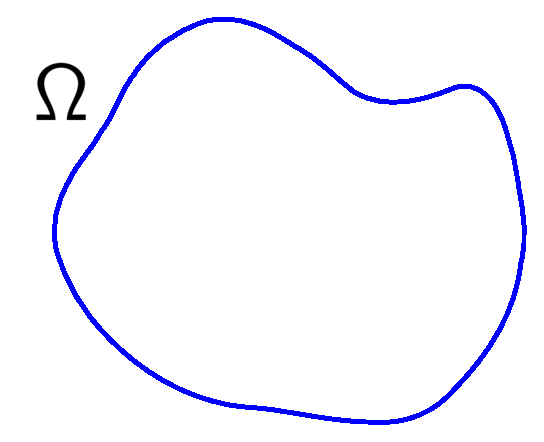
\includegraphics[scale = 0.45]{imgs/omega}}
%	\only<4>{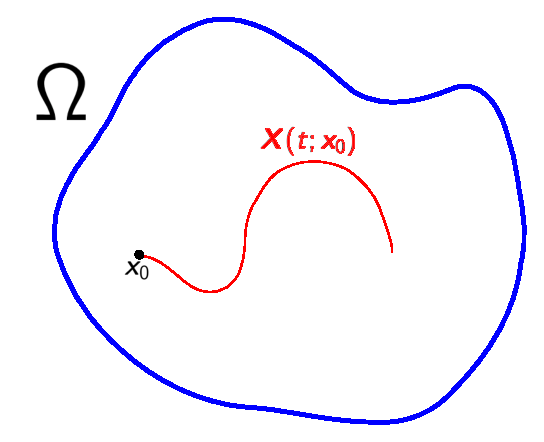
\includegraphics[scale = 0.45]{imgs/omega_traj}}
%\end{column}
%\end{columns}
%
%\end{frame}

\begin{frame}
\frametitle{Mathematical Formulation}
% Figures
\centering
\only<1>{\vspace{2mm}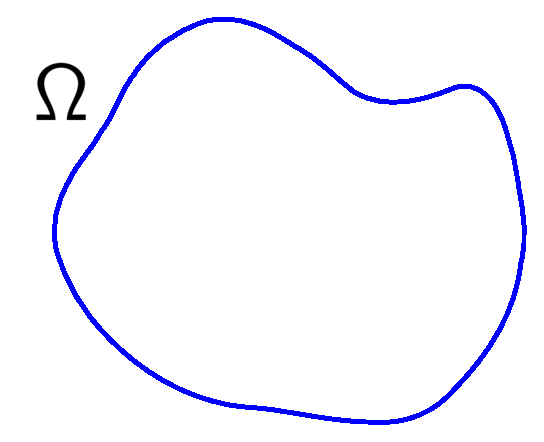
\includegraphics[height=0.6\textheight]{imgs/omega}}
\only<2>{\vspace{2mm}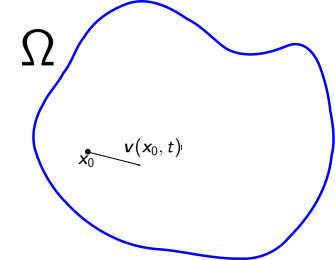
\includegraphics[height=0.6\textheight]{imgs/omega_vel}}
\only<3>{\vspace{2mm}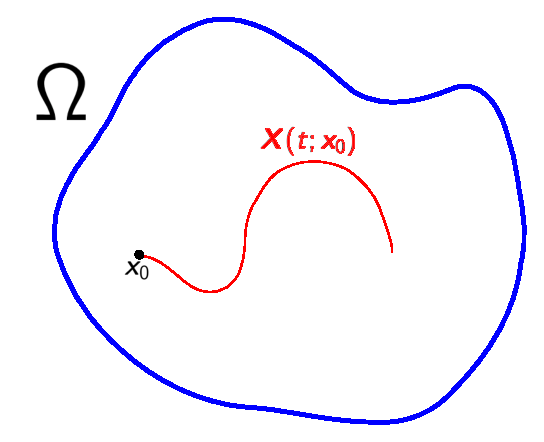
\includegraphics[height=0.6\textheight]{imgs/omega_traj}}
\end{frame}


%\begin{frame}
%	\frametitle{The Flow Region}
%	\begin{itemize}%%[<+->]
%		\item Flow domain \(\Omega \subset \R^2\).
%		\item Time interval of interest \([-T,T]\).
%	\end{itemize}
%\end{frame}
%
%
%\begin{frame}
%	\frametitle{Eulerian Description}
%	\begin{itemize}
%	\item Velocity function \(\bm{v}: \Omega\times[-T,T]\to \R^2\).
%	\end{itemize}
%\end{frame}
%
%\begin{frame}
%	\frametitle{Lagrangian Description}
%	\begin{itemize}%%[<+->]
%	\item Rather than describing the flow with a field, we are now interested in \textbf{individual} particle trajectories.
%	\item For initial position \(\bm{x}_0 \in \Omega\), the trajectory \(\bm{X}(t;\bm{x}_0)\) is the solution to
%	\[
%	\dpd{\bm{X}}{t} = \bm{v}(\bm{X},t); \quad \bm{X}(t_0;\bm{x}_0) = \bm{x}_0.	
%	\]
%	\end{itemize}
%\end{frame}




%\sectslide{Lagrangian Coherent Structures}

\begin{frame}
	\frametitle{Lagrangian Coherent Structures (LCSs)}
\begin{columns}[T,onlytextwidth]
	\begin{column}{.7\textwidth}
	\begin{itemize}[<+->]
		\item \textbf{Lagrangian} - patterns in particle trajectories.
		\item Wide range of diagnostic fields and techniques for extracting LCSs.
		\item Some look to partition \(\Omega\) into coherent regions.
	\end{itemize}
	\end{column}
	\begin{column}{.3\textwidth}
		\only<3>{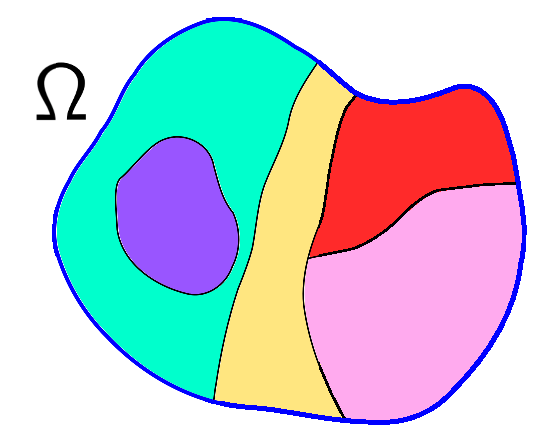
\includegraphics[scale = .45]{imgs/omega_partition}}
	\end{column}
\end{columns}
	\end{frame}


\begin{frame}
	\frametitle{Finite-Time Lyapunov Exponent (FTLE)}
	\begin{columns}[T,onlytextwidth]
	\begin{column}{.3\textwidth}
		\vspace{2.5mm}
		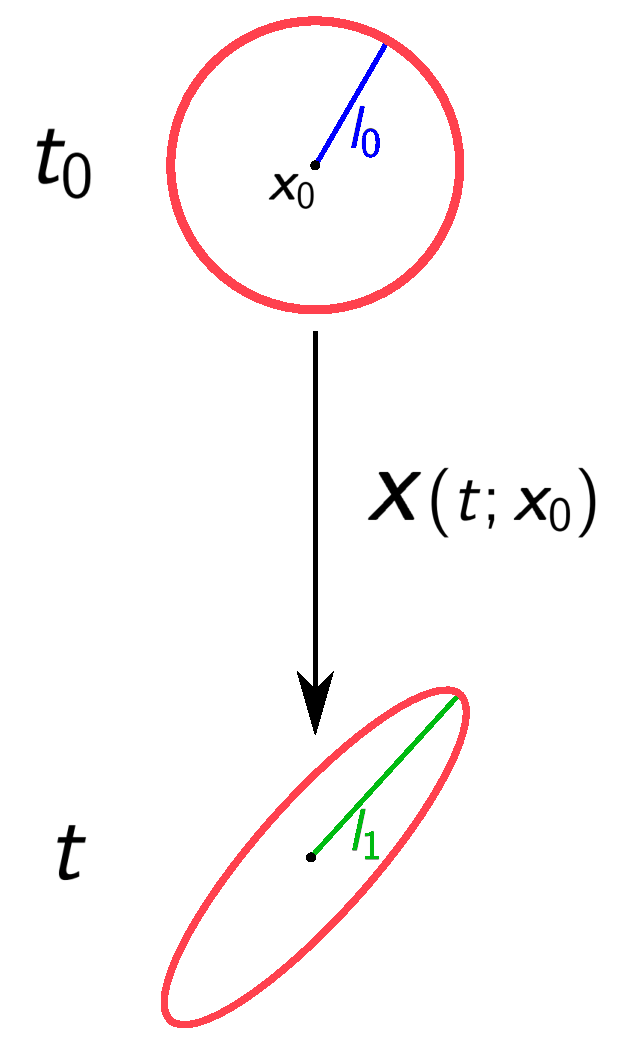
\includegraphics[scale=0.35]{imgs/ftle}
	\end{column}
	
	\begin{column}{.7\textwidth}
		\begin{itemize}
		\item Measure of maximal stretching of fluid.
		\[
		\sigma \coloneqq \frac{l_1}{l_0}
		\]
		\item One of the most common methods, established by \cite{shadden_2005_ftle}.
		\end{itemize}
	\end{column}
	\end{columns}

%		\[
%		\mathrm{FTLE}_{t_0}^{t}(\bm{x_0}) = \frac{1}{\abs{t - t_0}}\ln\sqrt{\lambda_{\text{max}}}.
%		\]
\end{frame}

\begin{frame}
\Wider[4em]{
\begin{center}
	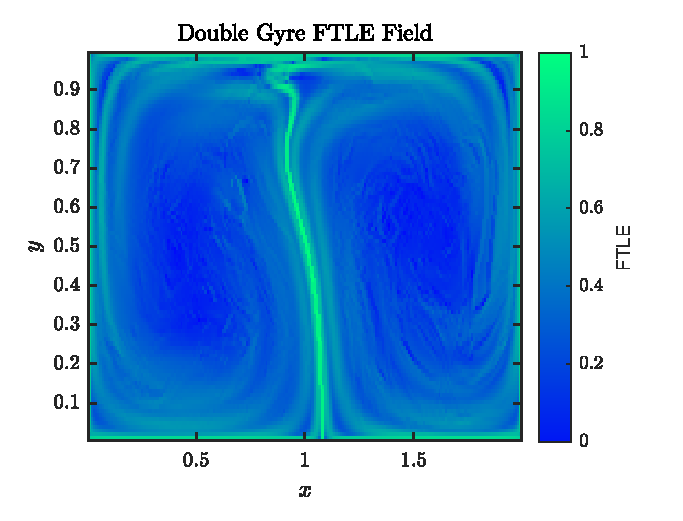
\includegraphics[width=0.48\textwidth]{../figures/doublegyre_ftle}%
	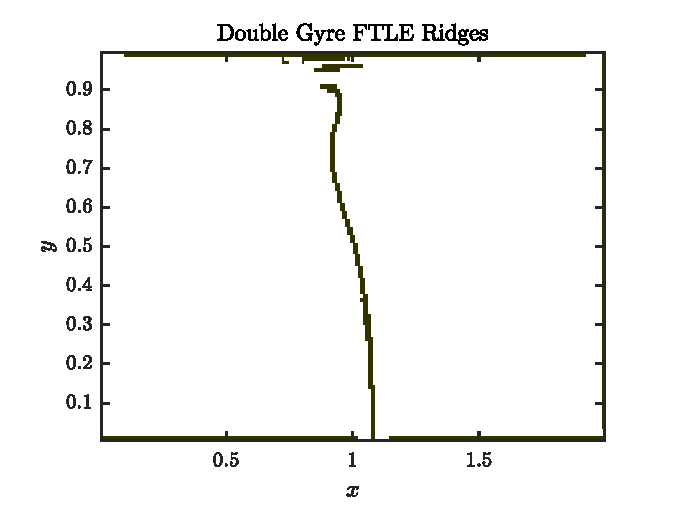
\includegraphics[width=0.48\textwidth]{../figures/doublegyre_ftle_ridges}
\end{center}
}
\end{frame}



\begin{frame}
	\frametitle{Lagrangian-Averaged Vorticity Deviation (LAVD)}
	\begin{itemize}[<+->]
		\item Vorticity measures local rotational rate.
		\item LAVD is the vorticity relative to spatial mean, averaged along trajectory, proposed by \cite{haller_2016_lavd},
	\end{itemize}


\end{frame}


\begin{frame}
\Wider[4em]{
	\begin{center}
	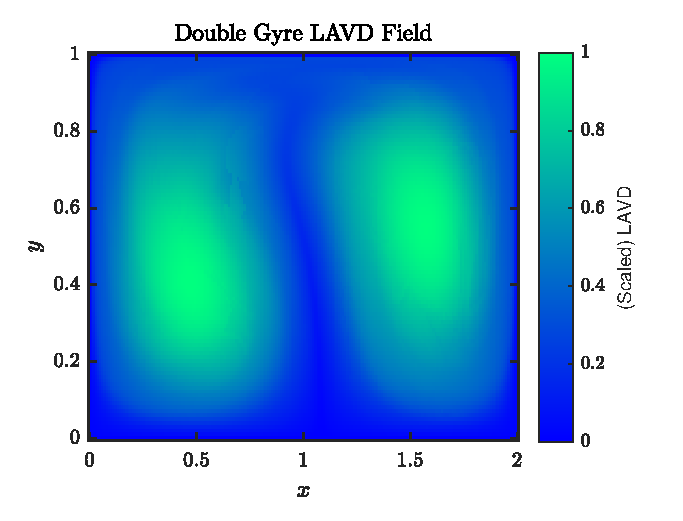
\includegraphics[width=0.48\textwidth]{../figures/doublegyre_lavd}%
	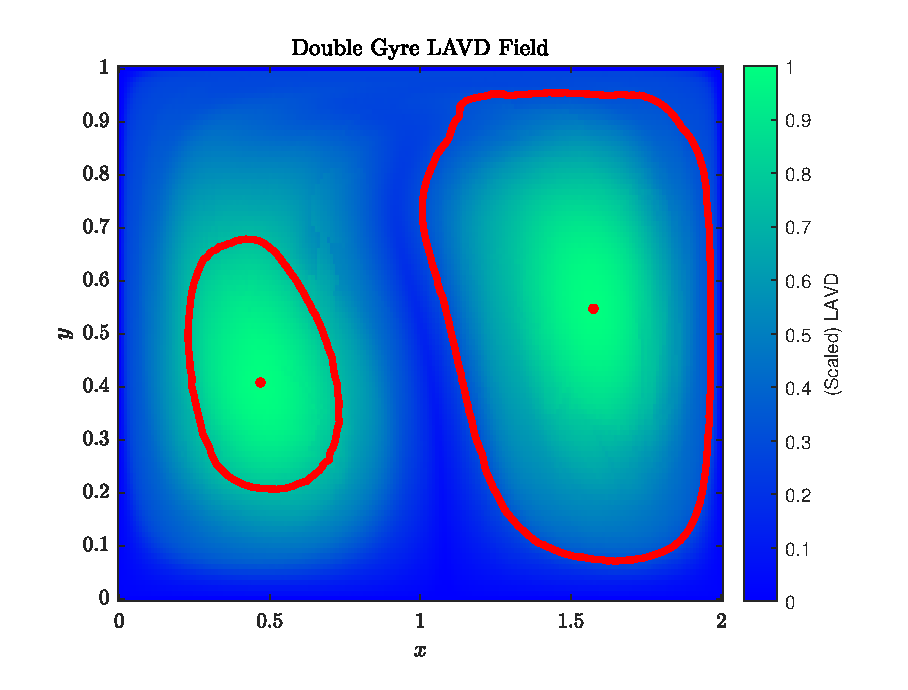
\includegraphics[width=0.48\textwidth]{../figures/doublegyre_lavd_contours}
	\end{center}
}
\end{frame}

\begin{frame}
\Wider[4em]{
\begin{center}
	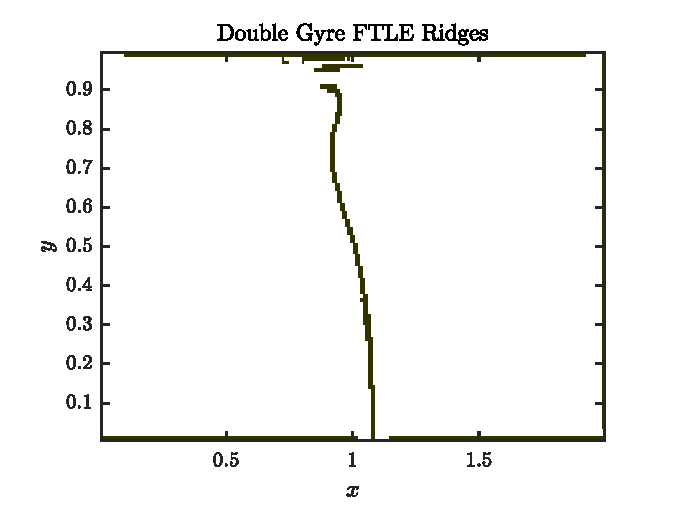
\includegraphics[width=0.48\textwidth]{../figures/doublegyre_ftle_ridges}%
	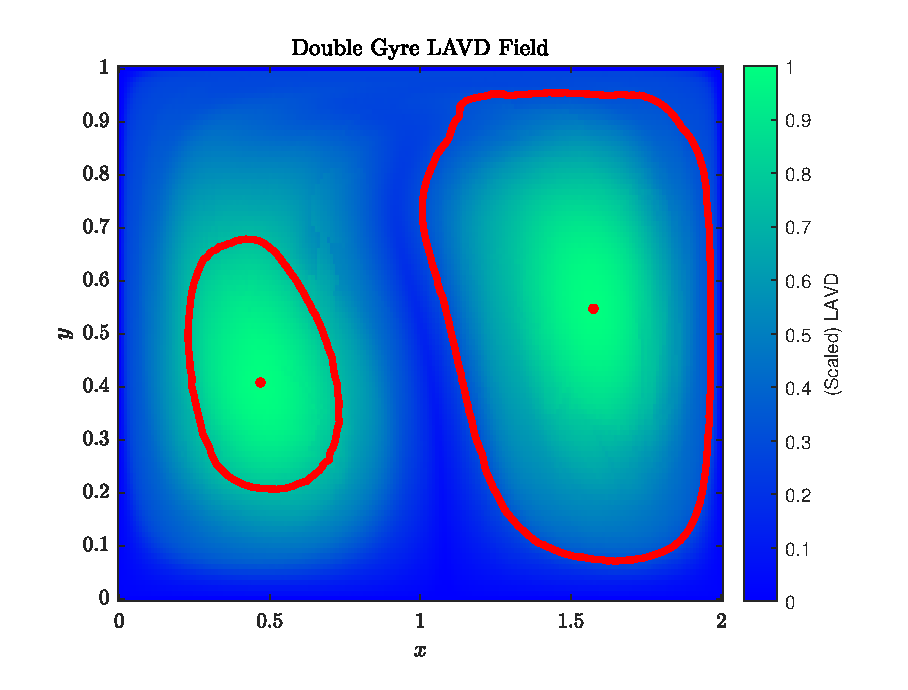
\includegraphics[width=0.48\textwidth]{../figures/doublegyre_lavd_contours}
\end{center}
}
\end{frame}

\begin{frame}
\frametitle{Questions}
\only<1-2>{Can we combine these perspectives into one way of looking at the flow?}

\vspace{5mm}
\only<2>{How does this look on real data?}
\end{frame}



\begin{frame}
\frametitle{The Real Data}

ANIMATION OF PARTICLES MOVING
\end{frame}


\begin{frame}
\centering
	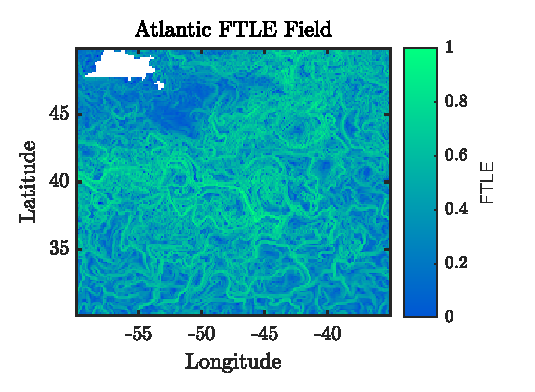
\includegraphics[width=0.9\textwidth]{../figures/atlantic_ftle}

\end{frame}


\begin{frame}
\centering
	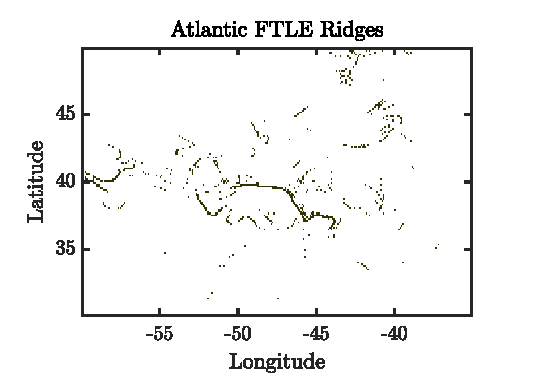
\includegraphics[width=0.9\textwidth]{../figures/atlantic_ftle_ridges}
\end{frame}


\begin{frame}
\centering
	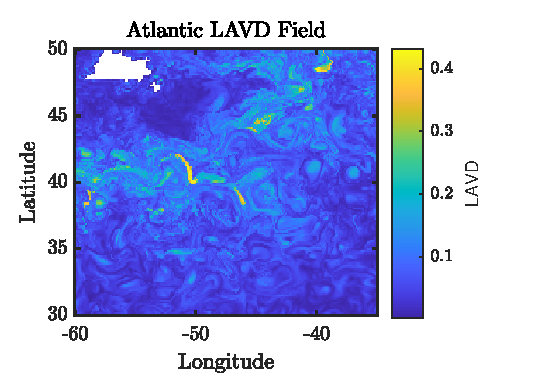
\includegraphics[width=0.9\textwidth]{../figures/atlantic_lavd}

\end{frame}

\begin{frame}
	\centering
	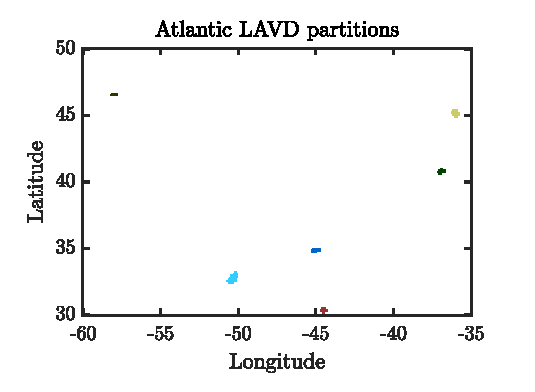
\includegraphics[width=0.9\textwidth]{../figures/atlantic_member_lavd}
\end{frame}

%\sectslide{Clustering}

%clustering is used to abstact away from the dynamical fields, so we stop worrying about exactly what we are extracting, just how we prtition the flow

%\begin{frame}
%	\frametitle{Intro to Clustering}
%	\begin{itemize}[<+->]
%	\item Data science problem: grouping similar points together into clusters.
%	\item A fuzzy clustering algorithms assigns membership probabilities.
%	\end{itemize}
%\end{frame}

\begin{frame}
	\frametitle{How Can We Combine Perspectives: Clustering}
	\begin{itemize}[<+->]	
	\item Grouping similar points together into clusters.
	\item Key idea: \textbf{any} partitioning of the flow is a clustering.
%	\item Consensus clustering combines different clusterings of the same data.
	\item Fuzzy consensus clustering combines different clusterings of the same data, proposed by \cite{wu_2017_fcc}.
	\end{itemize}
\end{frame}


\begin{frame}
\frametitle{}
\centering
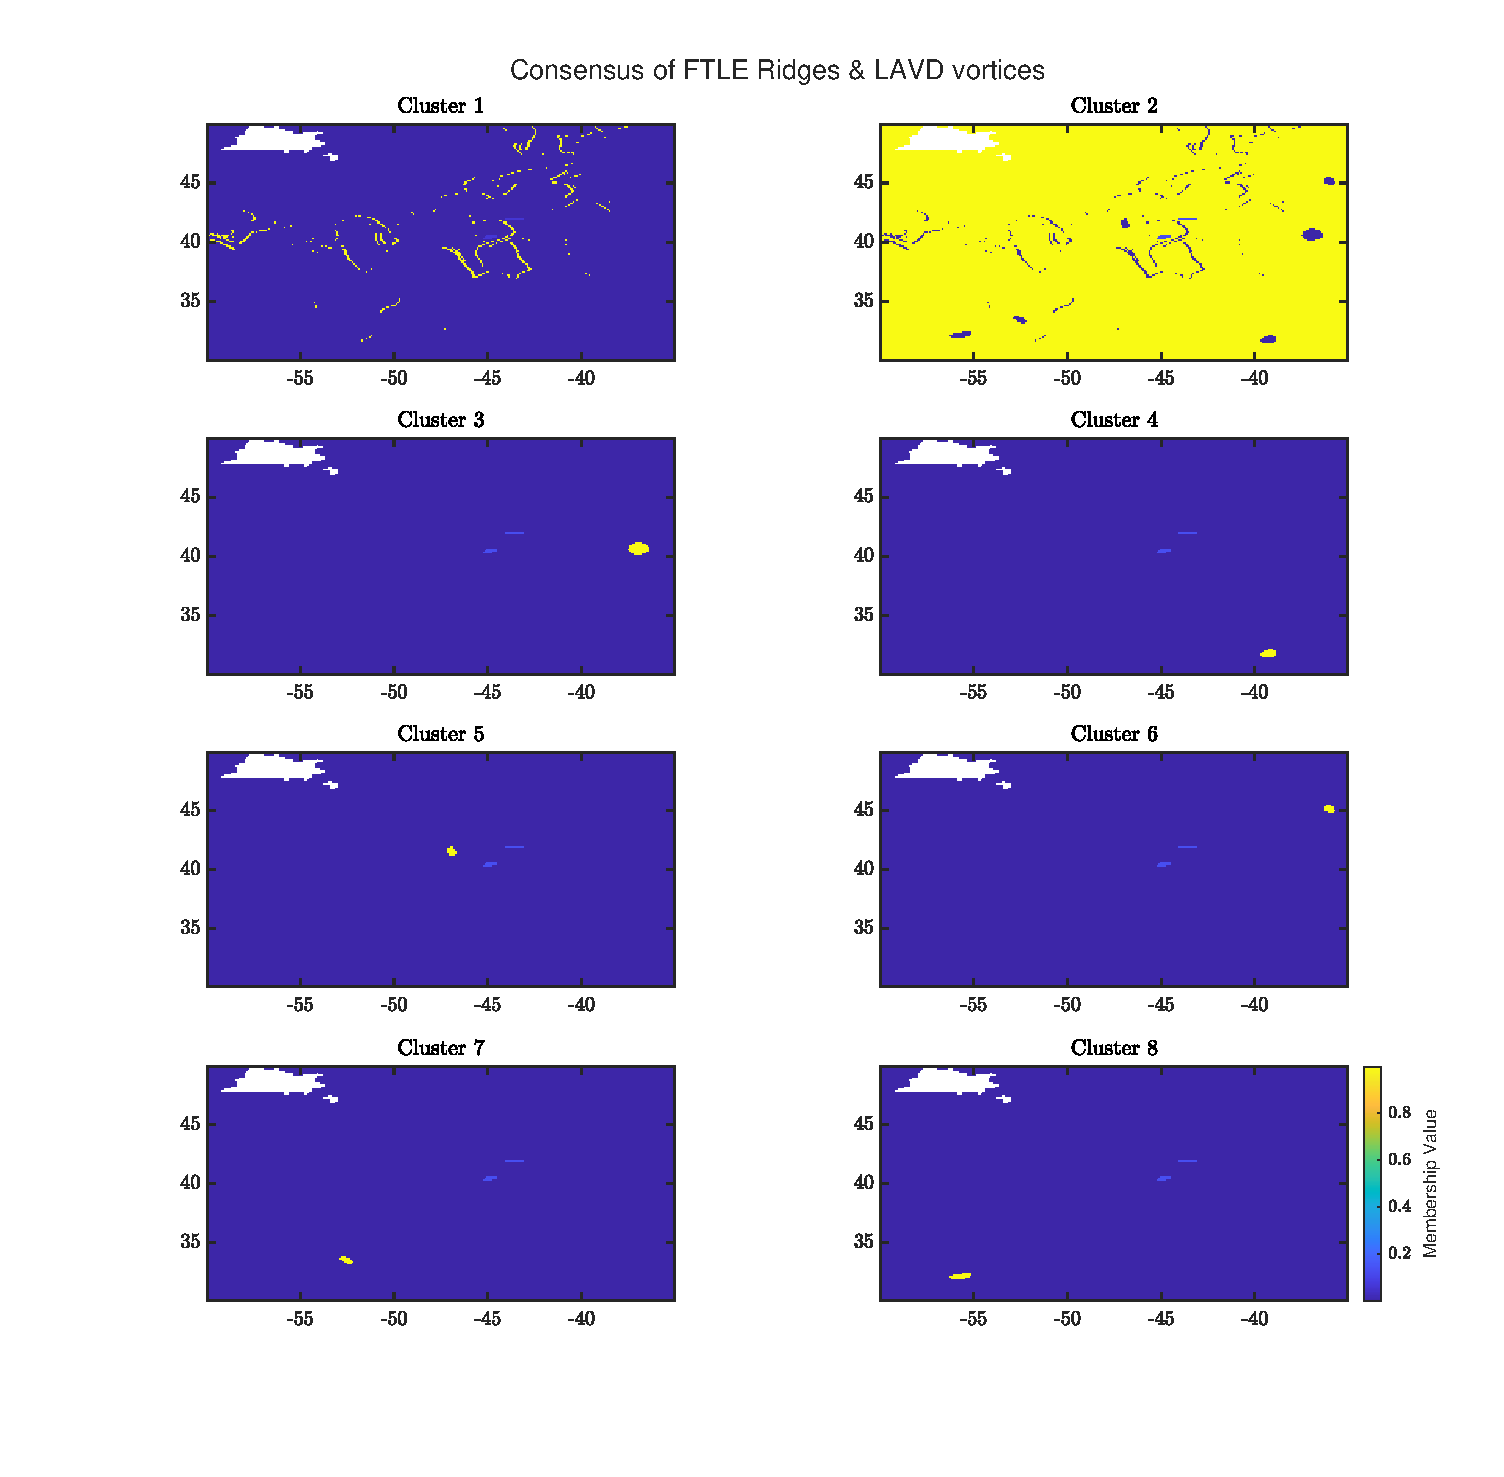
\includegraphics[height=0.89\textheight]{../figures/atlantic_cons_ftlelavd}

\end{frame}



%\sectslide{Application to Oceanographic Data}



\begin{frame}
	\frametitle{Temperature Field}
	\begin{itemize}[<+->]
	\item But coherency can extend beyond just the flow itself...
	\item Co-evolving variables such as temperature can reflect LCSs in flow or suggest their own coherency, from \cite{balasuriya_2018_glcs}.
	\end{itemize}
\end{frame}

\begin{frame}
	\centering
	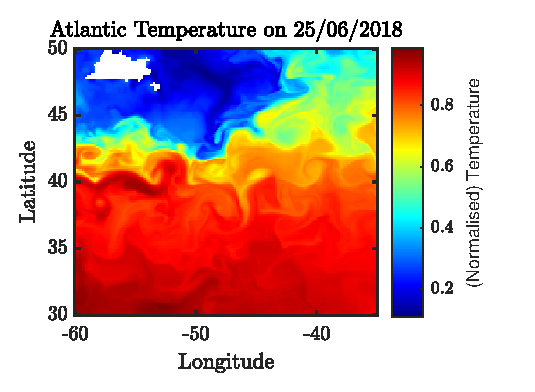
\includegraphics[width=0.9\textwidth]{../figures/atlantic_temp}
\end{frame}

\begin{frame}
\centering
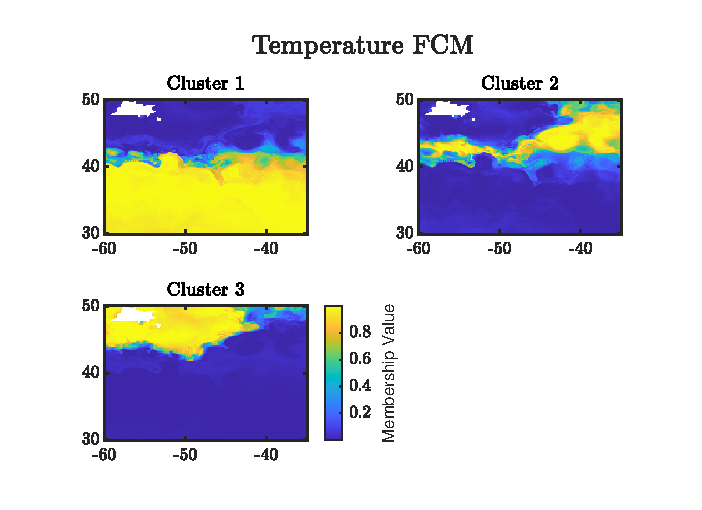
\includegraphics[width=1\textwidth]{../figures/atlantic_member_sst}
\end{frame}

%\begin{frame}
%	\frametitle{FCC Application}
%	\begin{itemize}
%	\item Three different perspectives on the flow.
%	\item Can we bring them together?
%	\end{itemize}
%\end{frame}

\begin{frame}
	\centering
	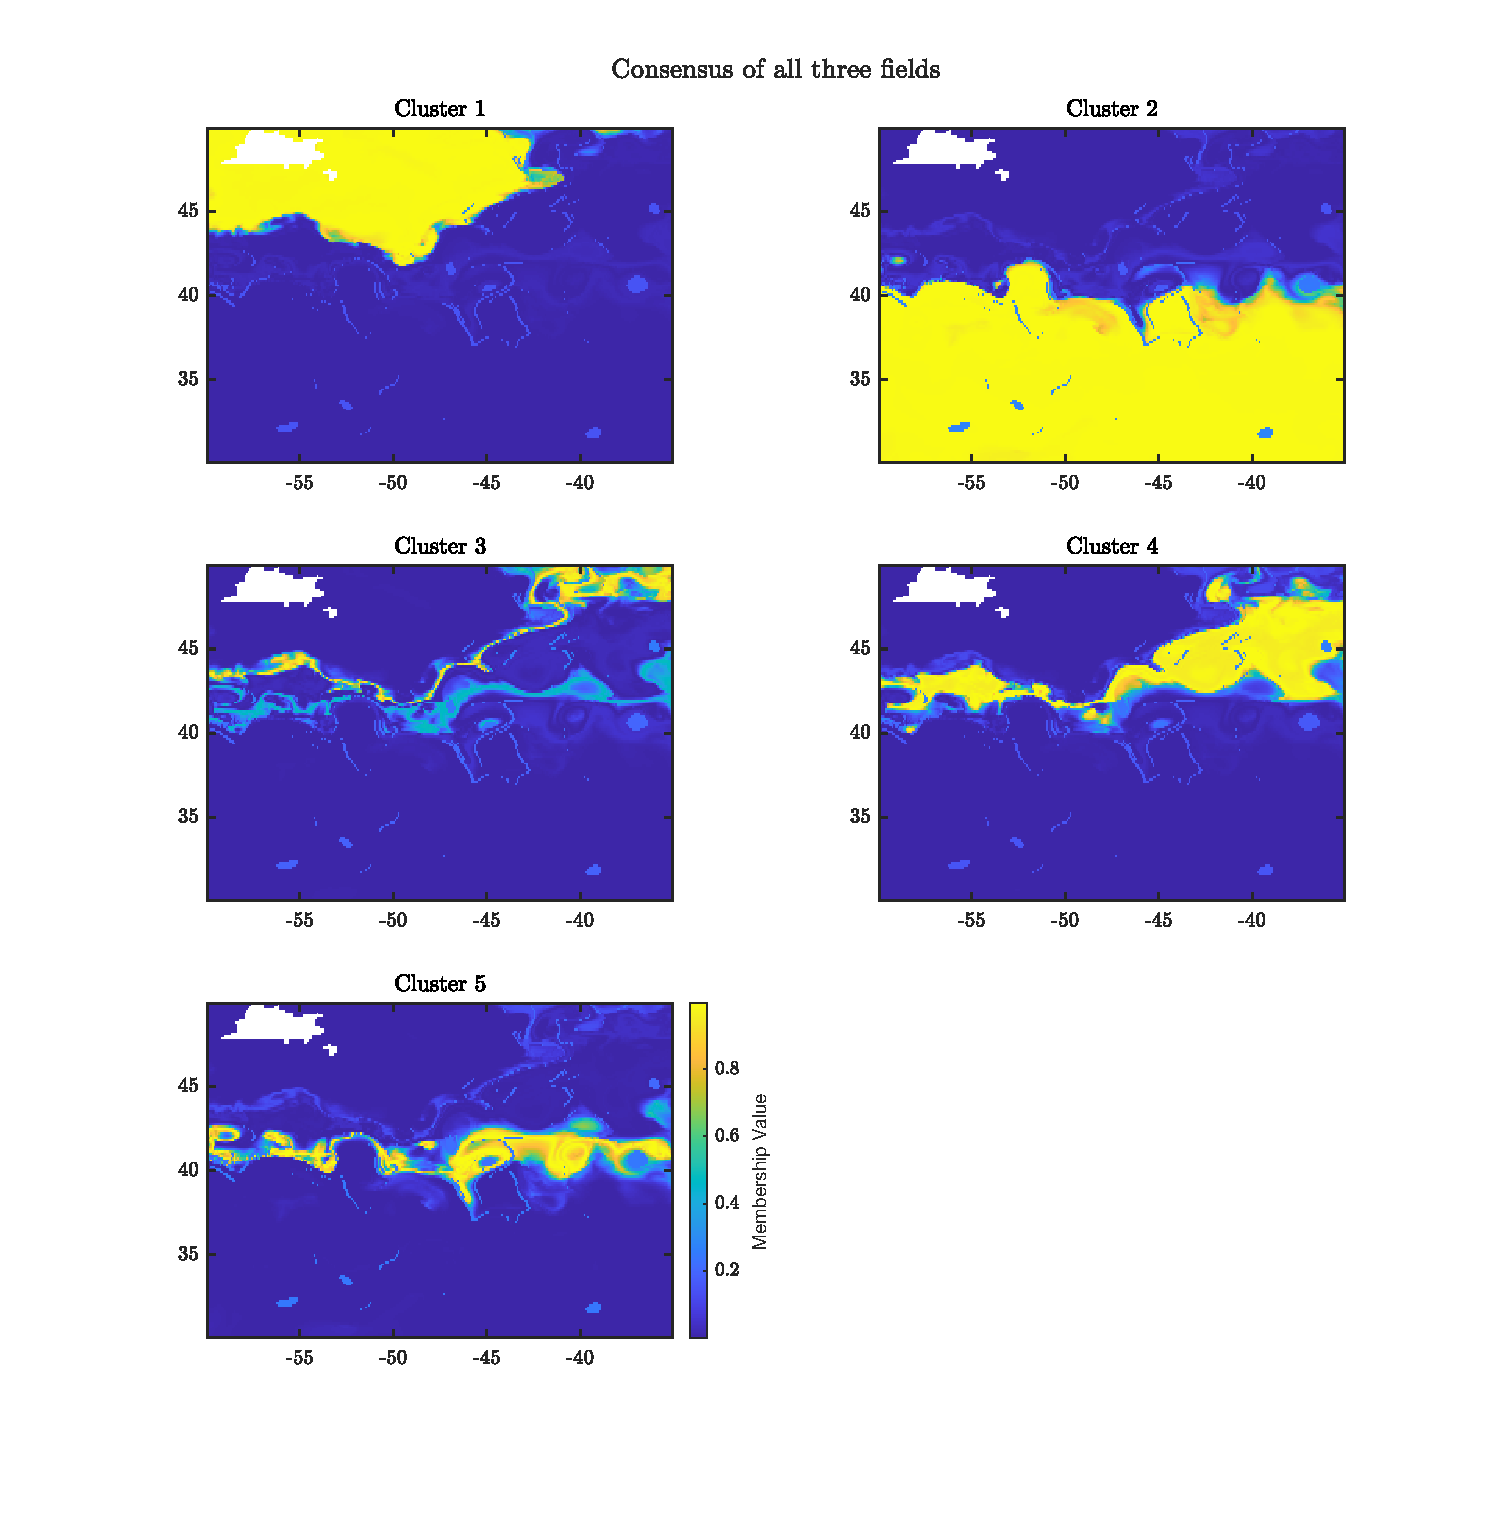
\includegraphics[height = 0.89\textheight]{../figures/atlantic_member_sensible}
\end{frame}

%\sectslide{Future Work \& Conclusion}

\begin{frame}
	\frametitle{Conclusions}
	\begin{itemize}	
	\item Combining FTLE \& LAVD is not quite right.
	\item Parameters are tricky.
	\item Addition of temperature was promising.
	\end{itemize}
\end{frame}



\begin{frame}
	\frametitle{References}
	\footnotesize
\bibliographystyle{apalike}
\bibliography{../notes/lcs_bib}
\end{frame}




\end{document}






%%% Local Variables: 
%%% mode: latex
%%% TeX-PDF-mode: t 
%%% TeX-master: t
%%% End: 